\documentclass[11pt]{article}

% load some asm stuff -
\usepackage{amssymb}
\usepackage{amsmath}
\usepackage{amsthm}
%\usepackage{palatino,lettrine}
\usepackage{fancyhdr}
\usepackage{epsfig}
\usepackage[round,comma,sort]{natbib}
\usepackage{simplemargins}
\usepackage{setspace}
\usepackage[margin=0pt,font=small,labelfont=bf]{caption}

\bibliographystyle{plos2009}

% Set the size
%\textwidth = 6.75 in
%\textheight = 9.75 in
%\oddsidemargin = 0.0 in
%\evensidemargin = 0.0 in
%\topmargin = 0.01 in
%\headheight = 0.0 in
%\headsep = 0.25 in
%\parskip = 0.15in
\doublespace

\setallmargins{1in}

\newtheorem{example}{Example}[section]
\newtheorem{thm}{Theorem}[section]
\newtheorem{property}{Property}[section]

\theoremstyle{definition}
\newtheorem{defn}[thm]{Definition}

\makeatletter
\renewcommand\subsection{\@startsection
	{subsection}{2}{0mm}
	{-0.05in}
	{-0.5\baselineskip}
	{\normalfont\normalsize\bfseries}}
\renewcommand\subsubsection{\@startsection
	{subsubsection}{2}{0mm}
	{-0.05in}
	{-0.5\baselineskip}
	{\normalfont\normalsize\itshape}}
\renewcommand\paragraph{\@startsection
	{paragraph}{2}{0mm}
	{-0.05in}
	{-0.5\baselineskip}
	{\normalfont\normalsize\itshape}}
\makeatother
\linespread{1.2}

\fancypagestyle{proposal}{\fancyhf{}%
	\fancyhead[RO,LE]{\thepage}%
	\fancyhead[LO,RE]{ChE 525 Understanding Maintenance Coefficients}%
	\renewcommand\headrulewidth{1pt}}
\pagestyle{proposal}

% Single space'd bib -
\setlength\bibsep{0pt}

\renewcommand{\rmdefault}{phv}\renewcommand{\sfdefault}{phv}

%\newboxedtheorem[boxcolor=black, background=gray!5,titlebackground=orange!20,titleboxcolor = black]{color_box_example}{Example}{test}

% Change the number format in the ref list -
\renewcommand{\bibnumfmt}[1]{#1.}

% Change Figure to Fig.
\renewcommand{\figurename}{Fig.}

%Joycelyn Chan, Joshua Lequieu, Michael Paull, Chidanand Balaji, Ryan Tasseff
%Our derivation follows closely the earlier development of Fredrickson \citep{Fredrickson:1976fk}.

% Begin ...
\begin{document}

%\begin{titlepage}
{\par\centering\textbf{\Large Understanding Maintenance Coefficients using Unstructured Models of Well-Mixed Cultures}}
\vspace{0.2in}
{\par \centering \large{Jeffrey D. Varner$^{*}$}}
\vspace{0.05in}
{\par \centering \large{School of Chemical Engineering$^{*}$}}
{\par \centering \large{Purdue University, West Lafayette IN 47907}}
\vspace{0.1in}
{\par \centering \small{Copyright \copyright\ Jeffrey Varner 2016. All Rights Reserved.}}\\

%\end{titlepage}
\date{}
\thispagestyle{empty}

\setcounter{page}{1}

%material and energy balances around the different processes cells do. For example, understanding how the abundance of raw materials in a bioreactor influences
%cell growth, or the production of valuable protein or small molecule products requires a materials balances around the major components of the system.
%The production of valuable small molecule or protein products requires large connected intracellular reaction networks that produce or consume energy.
%Thus, to understand the operation of biochemical systems and ultimately to manipulate them for societal gain,

\section*{Introduction}
Maintenance coefficients 
Fed-batch cultures are the most complex of the three operating modes of a bioreactor.
Feb-batch (or sometimes also called semi-batch) operation is the typical mode that bioreactors are operated in industrially (however there are a few exceptions).
Feb-batch requires $F_{in}\neq{0}$ and $F_{out} = 0$, where the $F_{in}$ trajectory, called the feeding profile, is adjusted to maximize some target objectives e.g.,
the final product \emph{titer} (the concentration of the desired product at the end of the run) or the
\emph{productivity} (the rate of product formation). Thus, fed-batch cultures are complex because they are dynamic and have volume change;
the working volume in the reactor increases thereby diluting the contents of the vessel.
In this lecture, we'll develop a mathematical description of
fed-batch cultures using the general material balances, and then explore the different modes of product formation in these industrially important cultures.

\subsection*{General model equations for fed-batch cultures.}
Let's start with the general material balances we derived previously:
\begin{eqnarray}\label{eqn-metabolite-dilution-dynamic}
	\frac{dC_{j}}{dt} &=& \sum_{s~=~1}^{\mathcal{S}}v_{s}D_{s}C_{j,s} + \left(\sum_{r~=~1}^{\mathcal{R}}\sigma_{jr}\hat{r}_{r}\right) + \left(\sum_{k~=~1}^{\mathcal{T}}\tau_{j,k}q_{k}\right)X  - \frac{C_{j}}{V}\frac{dV}{dt}\qquad j=1,2,\dots,\mathcal{M}\\
	\frac{dX}{dt} &=& \sum_{s~=~1}^{\mathcal{S}}v_{s}D_{s}X_{s}+\left(\mu - k_{d}\right)X - \frac{X}{V}\frac{dV}{dt}\\
	\frac{dV}{dt} &=& \sum_{s~=~1}^{\mathcal{S}}v_{s}\frac{\rho_{s}}{\rho}F_{s} - \frac{V}{\rho}\frac{d\rho}{dt}
\end{eqnarray}where the quantity $D_{s}$,  called a \textit{dilution~rate} (hr$^{-1}$), is given as:
\begin{equation}
	D_{s} \equiv \frac{F_{s}}{V}\qquad s=1,2,\dots,\mathcal{S}
\end{equation}The quantity $C_{j}$ denotes the concentration of the jth extracellular metabolite, $V$ denotes the working volume of the culture and $X$ denotes the cellmass.
In a fed-batch culture, there are in-flows, but no out-flow from the culture vessel; thus $D_{s^{-}} = 0$ where $s^{-}$ denote the set of outflow streams.
Because there is no out-flow, there is a volume change ($dV/dt > 0$), and all the dilution terms in the material balances are non-negative.
Volume change also requires that we keep the volume balance:
\begin{eqnarray}\label{eqn-metabolite-batch}
	\frac{dC_{j}}{dt} &=& \sum_{s~=~1}^{\mathcal{S^{+}}}v_{s}D_{s}C_{j,s} + \left(\sum_{r~=~1}^{\mathcal{R}}\sigma_{jr}\hat{r}_{r}\right) + \left(\sum_{k~=~1}^{\mathcal{T}}\tau_{j,k}q_{k}\right)X - \frac{C_{j}}{V}\frac{dV}{dt} \qquad j=1,2,\dots,\mathcal{M}\\
	\frac{dX}{dt} &=& \sum_{s~=~1}^{\mathcal{S^{+}}}v_{s}D_{s}X_{s} + \left(\mu - k_{d}\right)X - - \frac{X}{V}\frac{dV}{dt}\\
	\frac{dV}{dt} &=& \sum_{s~=~1}^{\mathcal{S^{+}}}v_{s}\frac{\rho_{s}}{\rho}F_{s} - \frac{V}{\rho}\frac{d\rho}{dt}
\end{eqnarray}

\subsection*{Analysis of a simple fed-batch culture.}
To better understand the dynamics of a fed-batch culture, let's simplify the general equations by assuming a Monod growth model \citep{Legout:2010aa}, a single limiting nutrient $S$, a single sterile input feed stream (s=1)
with similar density to the working volume, no density change as a function of time, stable substrate and product, and no maintenance utilization of substrate.
With these assumptions (and dropping the stream index from the dilution rate) the general fed-batch balances reduce to:
\begin{eqnarray}\label{eqn-metabolite-batch-simple}
	\frac{dS}{dt} &=& DS_{1} - \frac{1}{Y_{X/S}^{*}}\mu X - \frac{1}{Y_{P/S}}q_{p} X - \frac{S}{V}\frac{dV}{dt}\\
	\frac{dP}{dt} &=& DP_{1} + q_{p}X - \frac{P}{V}\frac{dV}{dt}\\
	\frac{dX}{dt} &=& \left(\mu - k_{d}\right)X - \frac{X}{V}\frac{dV}{dt}\\
	\frac{dV}{dt} &=& F\left(t\right)
\end{eqnarray}
If we substitute the volume balance into the substrate, product and cellmass balances, we arrive at the simplified system of equations:
\begin{eqnarray}\label{eqn-metabolite-fedbatch-simple}
	\frac{dS}{dt} &=& D\left(S_{1} - S\right) - \frac{1}{Y_{X/S}^{*}}\mu X - \frac{1}{Y_{P/S}}q_{p} X\\
	\frac{dP}{dt} &=& D\left(P_{1}- P\right) + q_{p}X\\
	\frac{dX}{dt} &=& \left(\mu - k_{d}\right)X - DX \\
	\frac{dV}{dt} &=& F\left(t\right)
\end{eqnarray}
where $\mu$ is given by:
\begin{equation}\label{eqn-monod-growth-model}
	\mu = \mu_{g}^{max}\left(\frac{S}{K_{g} + S}\right)
\end{equation} and we assume the Luedeking and Piret model for product formation \citep{Luedeking:2000aa}:
\begin{eqnarray}
	q_{p} = \alpha~\mu+\beta
\end{eqnarray}
The input volumetric flow rate function $F(t)$ is specified by the user; different functions (or parameters within typical functions such as an exponential feed function) strongly influence the performance of the culture.
The cellmass, substrate, product and volume balances are coupled nonlinear differential equations which can be solved numerically using common packages such as MATLAB or JULIA \citep{BEKS14}.

Let's consider no product formation ($\alpha,\beta= 0$), and a common feeding function, the exponential feed function:

\begin{equation}
	F\left(t\right) =
	\begin{cases}
      0 & t\leq T_{s} \\
      \theta_{o}\exp\left(\theta_{1}t\right) & t>T_{s}
   \end{cases}
\end{equation}
Fed-batch reactors are typically run in batch mode for the first few hours for example, until the initial amount of substrate in the reactor is consumed.
Following the start of the feed (denoted as feed-start or $T_{s}$), substrate is continuously added to the reactor and cells accumulate.
Fed-batch reactors typically show a bi-phasic growth pattern of fast followed by slow growth (Fig\ref{fig-fedbatch-no-product}).
Cellmass concentration decreases in fed-batch cultures both because of cell death and \textit{dilution}; after the feed start the working volume in the reactor \texite{increases} at rate proportional to feeding profile $F(t)$.
\begin{figure*}[!h]\centering
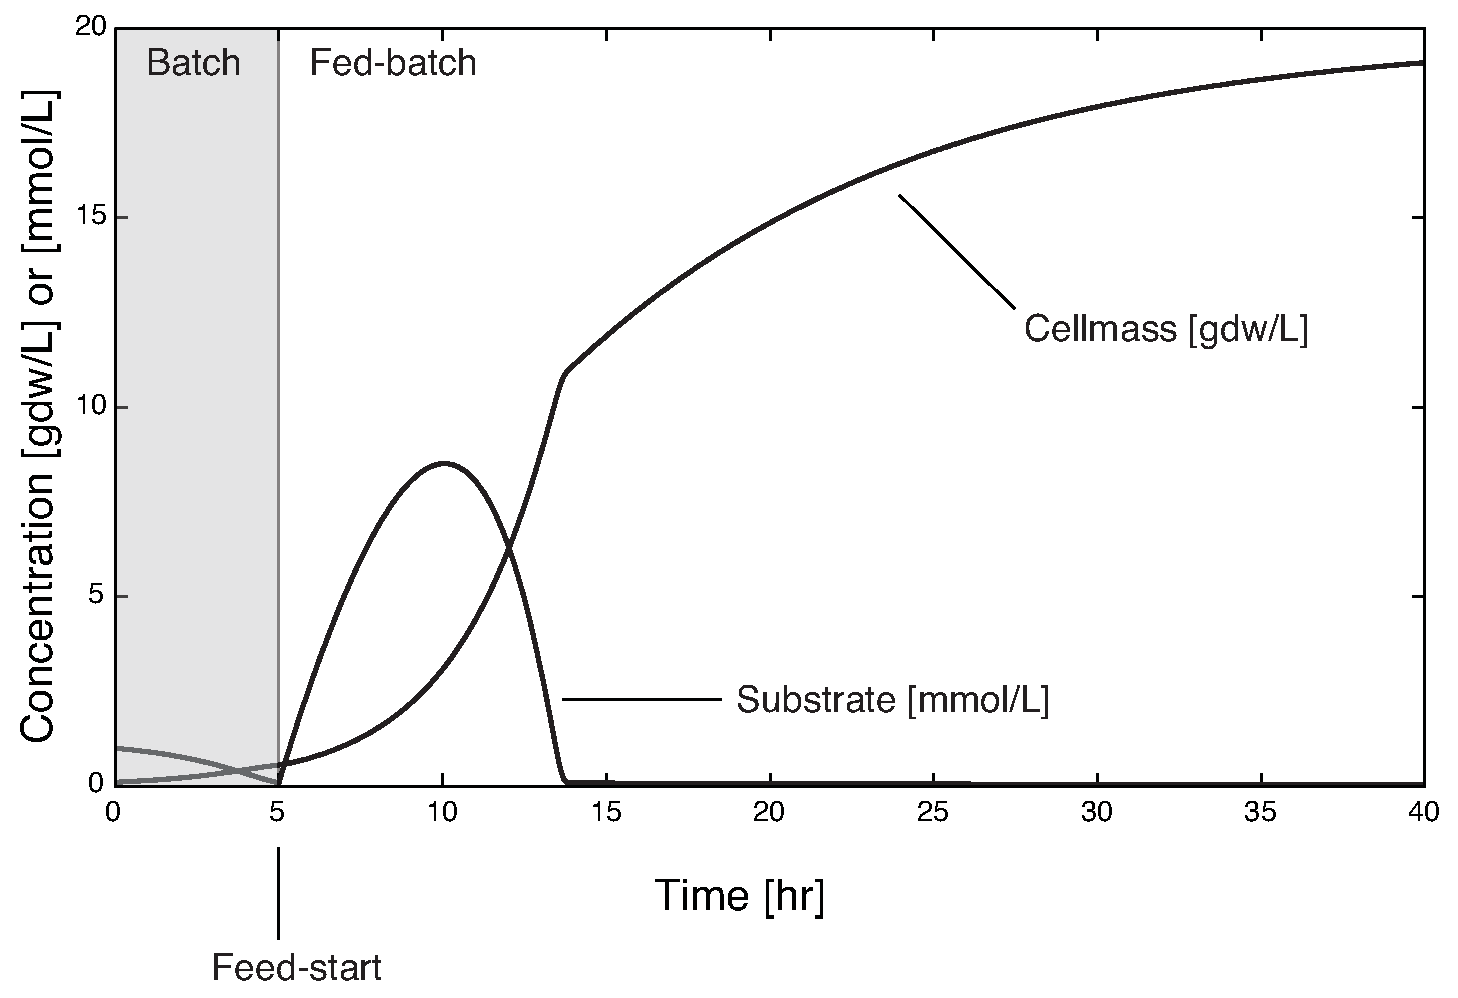
\psfig{file=figs/FedBatch-sims-eps-converted-to.pdf,width=0.8\textwidth}
\caption{Fed-batch growth of simple cells in a well-mixed bioreactor as a function of time with no product formation. The x-axis denotes the fermentation tile while the y-axis denotes the cellmass [gdw/L] or substrate [mmol/L] concentration.
The reactor is run in batch mode until the substrate is nearly exhausted, then the feed is started in the reactor. The feed-profile for this simulation is given
by a simple exponential ramp. }\label{fig-fedbatch-no-product}
\end{figure*}
Growth associated products ($\alpha = 1/Y_{X/P}, \beta = 0$) are produced when cells are actively growing, as a consequence of metabolic activity.
Typical growth associated products are organic acids such as Acetate, Lactate, Succinate or Ethanol (Fig. \ref{fig-fedbatch-gw-product}).
Non growth associated products ($\alpha = 0, \beta \neq 0$) are produced only after cell growth has slowed.
Typical non-growth associated products (also called secondary metabolites) are antibiotics such as Penicillin (Fig. \ref{fig-fedbatch-ngw-product}).

\begin{figure*}[!h]\centering
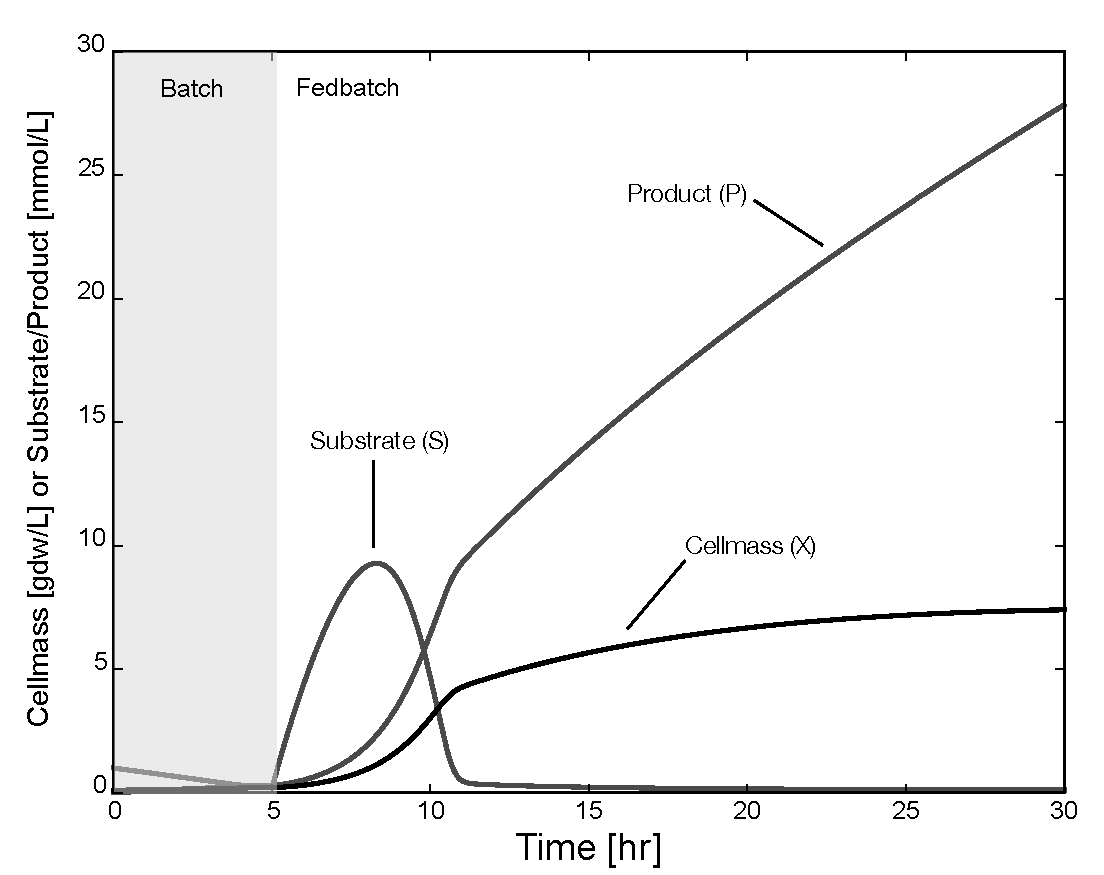
\psfig{file=figs/FB-GrowthAsscoaited-ChE525.pdf,width=0.8\textwidth}
\caption{Fed-batch growth of simple cells in a well-mixed bioreactor as a function of time with growth associated product formation. The x-axis denotes the fermentation tile while the y-axis denotes the cellmass [gdw/L] or substrate [mmol/L] concentration.
The reactor is run in batch mode until the substrate is nearly exhausted, then the feed is started in the reactor. The feed-profile for this simulation is given
by a simple exponential ramp.}\label{fig-fedbatch-gw-product}
\end{figure*}

\begin{figure*}[!h]\centering
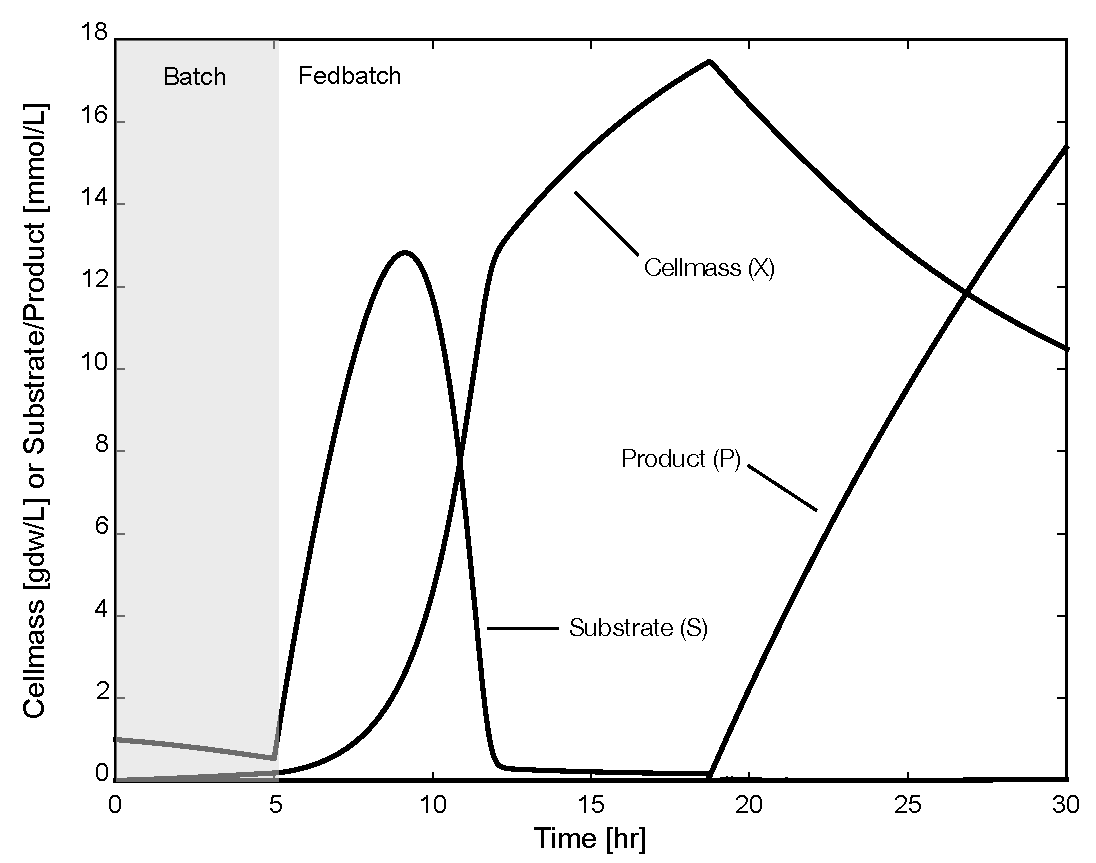
\psfig{file=figs/FB-NonGrowthAssociated-ChE525.pdf,width=0.8\textwidth}
\caption{Fed-batch growth of simple cells in a well-mixed bioreactor as a function of time with secondary product formation. The x-axis denotes the fermentation tile while the y-axis denotes the cellmass [gdw/L] or substrate [mmol/L] concentration.
The reactor is run in batch mode until the substrate is nearly exhausted, then the feed is started in the reactor. The feed-profile for this simulation is given
by a simple exponential ramp.}\label{fig-fedbatch-ngw-product}
\end{figure*}

\clearpage

\bibliography{Notes}
\end{document}
